Although this is called the intro, I've also but int bits that I want to put in that are general for more than one chapter. These are just bullet pointed \emph{aide memoirs} at the moment but will obviously be fleshed out in time.

\section{Statistical Ecology}

Some general remarks about stat ecol perhaps.

\section{Themes}

\bi
	\item Morphing
	\item Modifying penalties
	\item Computational efficiency
	\item Realistic physical models!!!!!!
\ei


\section{Some notational conventions}



\section{Generalized Additive Models}

General GAM setup. The is will mostly be taken from \cite{simonbook}, \cite{rwc} and \cite{marraradice2010}.

\bi
\item Splines
\item objective function
\label{GAMobjfcn}
\item penalties
\label{GAMpenalties}
\item bases - TPRS (and maybe P-splines?)
\item fitting - GCV REML etc
\item other stuff - MSE, EDF etc
%	\bi
%	\item MSE
%	Mean squared error is... (look at HTF)
%	
%	\begin{equation}
%\text{MSE}(\hat{f}) = \frac{1}{P} \sum_{j=1}^P (\hat{f}(x_j) - z_j)^2,
%\end{equation}
%the mean difference between the model ($\hat{f}$) evaluated at the prediction points ($\{x_j : j=1 \dots P\}$) and the true value of the function ($\{z_j : j=1 \dots P\}$.) This gives the MSE per model, since here many realisations are run, the mean of these over all simulations is taken and the standard error is calculated.
%	\item EDF
%	
%The estimated degrees of freedom gives an measure of the complexity of the model that was fit to the data. The higher the EDF, the more basis functions were used and  the more complex the model.  Since the models used here are penalised, it is the penalty term that controls the overall ``wigglyness'' of the spline and hence the EDF. Although the basis dimension is set in the model, this is just an upper bound, the smoothing penalty suppresses parts of the model. Therefore basis dimension is not a major concern provided that it is not set too low (\cite{simonbook}, p. 161.) 
%
%	\ei
\ei

\section{Finite area smoothing}

\subsection{Overview of finite area smoothing}

Splines are a popular way of performing spatial smoothing in two dimensions. In this context, they are often used to fit smooth functions over a geographical region. A typical application of this is in ecological modelling; a response (be it location of individuals in a population or concentration of a chemical) is modelled as a function of its spatial coordinates. The estimated function can then be used to perform inference on the population, whether that be an abundance estimate, density map or a more sophisticated inferential goal. Finite area smoothing simply specifies that the domain over which this smoothing takes place is bounded.

When the geographical region has a \emph{complex boundary}, features from one part of the domain can unduly influence other parts. Considering the boundary as a polygon, a complex boundary is a non-convex polygon, in particular when the non-convexity is relatively extreme. Often this consists of having some peninsula-like feature(s) in the domain with notably different observation values on either side of the feature. Given that there is some scientific motivation as to why those parts of the domain should not affect each other, features such as peninsulae give rise to a phenomenon known as \emph{leakage}.

Leakage occurs when a smoother inappropriately links two pats of a domain (\cite{soap}). The phenomenon is problematic since it causes the fitted surface to be mis-estimated; this can then lead to incorrect inference (eg. biased abundance estimates), which is clearly not desirable. Leakage can be seen in \fig{leakage} where the high values in the upper half of the domain leak across the gap to the lower values below and vice versa.

% leakage example 
\begin{figure}
\centering
% trim order l b r t
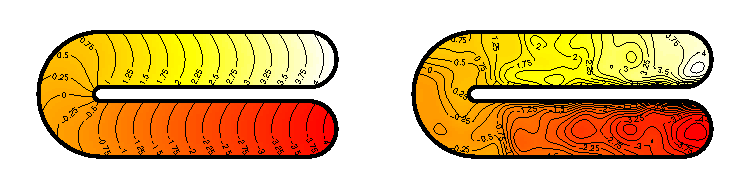
\includegraphics{intro/figs/ramsay-leak.pdf}\\
\caption{An example of leakage. A thin plate regression spline was fit to data sampled from the function on the left, here the model smooths across the gap in the middle of the domain (right.)}
\label{leakage}
\end{figure}

The problem of leakage arises because of the way in which the smoother defines how near objects are to one another. Most smoothing techniques use the Euclidean metric to measure the distance between data. Clearly though, this approach is a flawed: biological populations do not conform to Euclidean geometry in their movement patterns and hence their observed positions will reflect this. Just as whales no not uniformly distribute themselves across sea and glacier, fish do not lay their eggs on land. Natural and man-made barriers carve up the landscape (and seascape), partitioning biological populations; our models should take this into account.

The distribution of the population is smooth, just not necessarily over $\mathbb{R}^2$ (\cite{wangranalli}). Instead the structure of the domain that is under investigation must be modelled (implicitly or explicitly) for the correct inference to be drawn.

\subsection{Ramsay's horseshoe function as a benchmark for finite area smoothing}

\cite{ramsay} proposes a function which can be used to benchmark new approaches to 2-dimensional smoothing. The function takes the form of a horseshoe shape which is flat across the domain has a gradient along the domain's major axis. This can be seen in \fig{orig-fs}. \cite{soap} modifies the test function by adding curvature across the minor axis of the shape. This was added in order to avoid the horseshoe function lying in the nullspace of their model's penalty, making the problem trivial. It is the second shape that will be used for simulations here and shall be referred to as the \emph{Ramsay horseshoe} throughout; it is shown in \fig{leakage}.

% original horseshoe from Ramsay's paper
\begin{figure}
\centering
% trim order l b r t
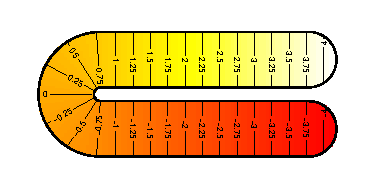
\includegraphics{intro/figs/orig-fs.pdf}\\
\caption{The horseshoe function as it appeared in \cite{ramsay}.}
\label{orig-fs}
\end{figure}

The test function highlights leakage well. As mentioned above, when the smoothing problem is specified in Euclidean distance, the model takes the distance between the points in the two arms of the horseshoe is the distance over the gap in-between them, rather than the distance along the major axis of the shape. This causes the high function values from one side to contaminate the other side (and the low to contaminate the high.) It is easy to see that this causes the smooth to be calculated incorrectly.
		
\subsection{Previous approaches to leakage}

The cause of leakage can be characterised in two ways: either the smooth does not respect the boundary of the domain, or the smooth does not take into account the geometry of the domain (in particular with regard to the distance between points within the domain). Previous work in this area has been to combat leakage along these two lines. Work of \cite{ramsay} and \cite{soap} both use a PDE boundary condition approach to try to prevent leakage, where as \cite{wangranalli} and \cite{eilerstalk}  attempt to approximate the intrinsic structure of the domain while not treating the boundary as something special in the basis setup. These four main works may be summarised as follows:

\begin{enumerate}
\item \cite{ramsay} proposes finite element $L$-splines (FELSPLINEs). The $L$-spline replaced the penalty term (see \secref{GAMpenalties}) with:
\be
\int_\Omega (L_p f)^2 \text{d}\Omega,
\ee
where $L_p$ is a roughness operator defined as:
\be
L_p=\Delta^p+c_{p-1}\Delta^{p-1}+\dots+c_1\Delta+c_0I.
\ee
Here $I$ is the identity operator, the $\{c_0,\dots, c_p\}$ are constants and the $\Delta$ is the Laplacian ($\Delta f = f_{xx}+f_{yy}$ in the usual notation). Although any differential operator could, in principle, be used for $L_p$, the Laplacian gives rise to a set of polynomials which are rotation and translation invariant which is clearly sensible given the objective function solution should not depend on the coordinate system used.

The PDE in the penalty cannot be analytically solved in two dimensions. Ramsay takes a finite element approach and triangulates the domain. He then constructs a set of bivariate quadratic polynomial basis functions over each triangle, specifying that there be continuity over the edges of the triangles. The union of these functions is then a solution to the PDE in the penalty and therefore the solution to the usual smoothing objective function (see \secref{GAMobjfcn}).

Since the triangulation and hence the penalty of the FELSPLINE is only calculated over the domain, and the continuity is specified over neighbouring cells, the method prevents leakage. Howevr, although FELSPLINE does not exhibit leakage on the original horseshoe (as in \fig{orig-fs}), in practice the model makes unrealistic physical assumptions. The boundary conditions of FELSPLINE specify that the gradient is zero, along normals to the boundary. This is not always physically realistic and as \cite{soap} show, by adding a small amount of curvature to the gradient of the Ramsay horseshoe the FELSPLINE performance begins to falter.

FELSPLINE does not offer a realistic physical model and is therefore not a viable solution to the finite area smoothing problem in general.

\item \cite{wangranalli} adopt a ``within-area distance'' formulation for thin plate splines. They take the geodesic distance between two points, that being the shortest path within the domain. This gives a definition of how near objects are in the domain. 

Since geodesic distance is only know if the true, intrinsic structure of the domain is known (which is effectively not possible), an approximation is used. Wang and Ranalli first create a weighted, undirected graph ($G$, say) with a data point at each vertex and the distance between each pair of vertices as the weights on the edges. They then take the restricted graph of $G$, $G_k$, in which each vertex is only connected to its $k$ nearest neighbours. With this new, restricted graph the geodesic distances between each pair of vertices can be calculated using Floyds algorithm.

As the authors point out, the quality of the approximation is dependent on the size of the data set and its density. At low densities the estimated geodesic distance will tend towards the Euclidean, at high densities the approximation tends, asymptotically toward the true geodesic distance (\cite{bernstein}). Even if  dense enough data were available, the method will be rather slow since Floyd's algorithm is cubic in the number of vertices (the size of the data set). Finally, although the $k$-nearest neighbours algorithm used is not specified in the paper, in general such procedures are computationally expensive, adding another source of impedance to the technique.

Taking these points into account, Wang and Ranalli's approach appears cumbersome, slow and dependent on dense data.

\item \cite{soap} consider constructing a soap film over the domain. The film is then distorted smoothly by the data while minimizing the surface tension in the film. The domain ($\Omega$) is bounded by some polygon with known or estimated boundary conditions (in practice these are estimated by a cyclic spline).

Mathematically, the soap film smoother is constructed by first specifying a set of functions $\rho_k(x,y)$, which are each solutions to the Laplace equation in two dimensions:
\be
\frac{\partial^2\rho}{\partial x^2} + \frac{\partial^2\rho}{\partial y^2} = 0
\ee
except at one of the knots ($x^*_k,y^*_k$). Then, solving Poisson's equation in 2-dimensions:
\be
\frac{\partial^2 g_k}{\partial x^2} + \frac{\partial^2 g_k}{\partial y^2} = \rho
\label{soap-poisson}
\ee
with $\rho=\rho_k(x,y)$, where $k$ indexes the knots, the set of basis functions for the soap film smoother, $g_k(x,y)$ is found, along with $a(x,y)$ (the solutions to \eqn{soap-poisson} when $\rho=0$). These bases are then summed to form:
\be
f=a(x,y)+\sum_{k=1}^n \gamma_k g_k(x,y),
\ee
the soap film smoother, where the $\gamma_k$ are parameters to be estimated. The (isotropic) penalty term (\secref{GAMpenalties}) is:
\be
\int_\Omega \Big(\frac{\partial^2 f}{\partial x^2}+\frac{\partial^2 f}{\partial y^2} \Big)^2\text{d}x\text{d}y,
\ee
Differing from the standard \tprs penalty since (\emph{i}) the integration occurs only over $\Omega$, (\emph{ii}) there is no mixed derivative term, and (\emph{iii}) the whole integrand is squared rather than each term individually. This allows the $x$ and $y$ term's derivatives to be traded off against each other so the nullspace of the penalty is infinite dimensional. This allows those functions in the nullspace to be sufficiently wiggly to meet any boundary conditions.

The solution of the PDEs above, yielding the basis and penalty, is the most computationally expensive part of the procedure. Knots to use for $x_k^*$ and $y_k^*$ must be specified, usually using a grid. Numerical problems occur when knots are placed in boundary cells in the PDE solution grid.

Although mathematically elegant, the soap film smoother is a rather complex model. It also treats the boundary as a special case and uses a cyclic spline in order to approximate the boundary values. This treatment of the boundary seems rather unnatural...

\item An alternative approach to treating the boundary as something special is to transform the space in which the points lie to instead lie in a different domain which is more suitable for smoothing. For example, with Ramsay's horseshoe, it seems intuitive to simply bend the horseshoe into a long strip and then smooth on that domain.

Indeed, \cite{eilerstalk} proposed using the \sch transform for this very purpose (I, independently, came to this method in 2008 via my obsessive listening to BBC Radio 4.) Using the \sch transform for smoothing will be elaborated on in chapter \ref{chap-sc}, so only a brief summary is given here.

The basic idea is to find a function, $\phi$ say, that takes points in the domain the data lie in ($W$) and maps them to a domain ($W^*$) in which the boundary is less complex ($\phi : W \rightarrow W^*$, mathematically).

Creating some kind of mapping between the space in which the data lies and the space in which conventional smoothers perform well is convenient. Not having to setup a new basis structure and relying on long tested methodology is clearly appealing. This approach also benefits from not treating the boundary as a special in the basis setup.
\end{enumerate}

Chapters \ref{chap-sc} and \ref{chap-mds} expand on the ideas in the last method; of using a transformation of space and conventional smoothers to solve the problem of leakage in finite area smoothing.

\section{Distance sampling}

This will be a very brief introduction to distance sampling methods, in the style of the encyclopaedia of environmetrics article.
